\documentclass[border=4pt]{standalone}
\usepackage[T1]{fontenc}
\usepackage{lmodern}
\usepackage{tikz}
\usetikzlibrary{positioning,arrows.meta}
\begin{document}
\sffamily\footnotesize
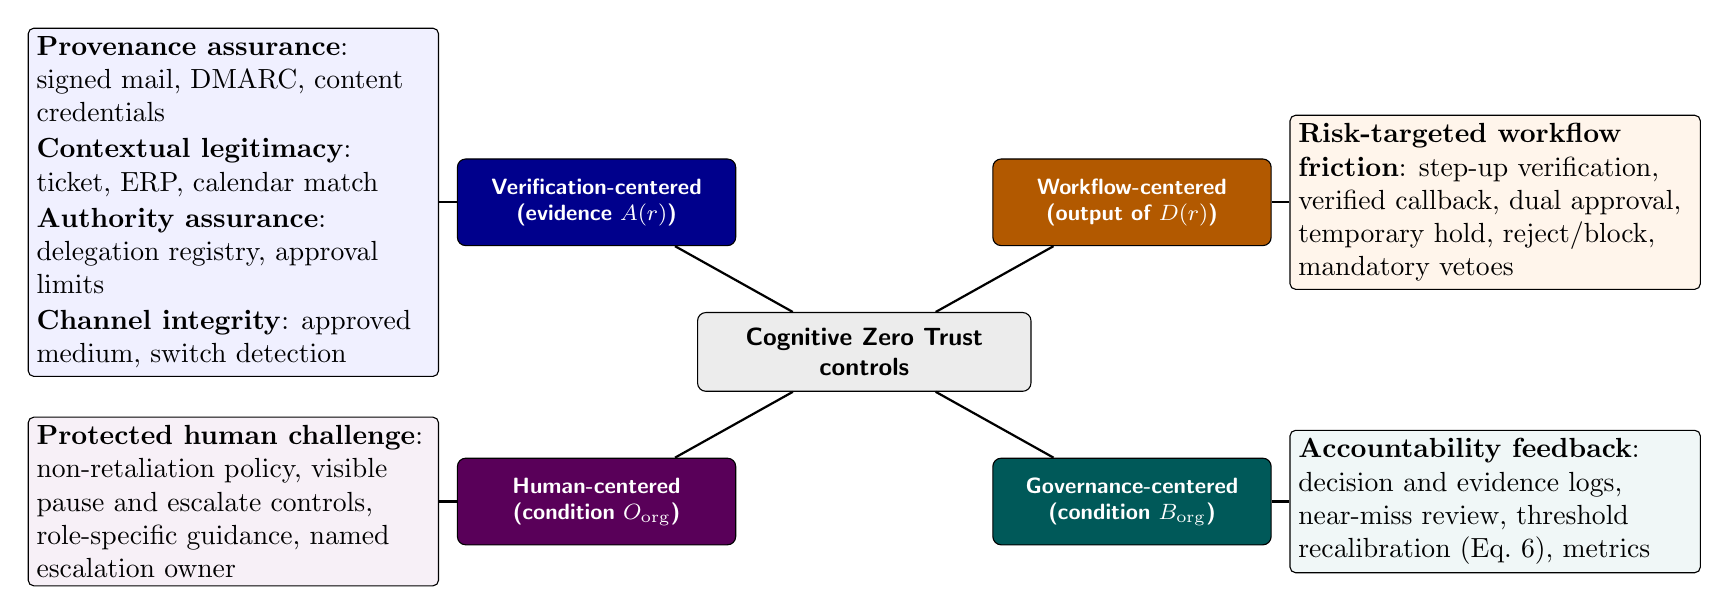
\begin{tikzpicture}[
  grp/.style={draw, rounded corners=3pt, align=center, text width=33mm, minimum height=11mm, font=\sffamily\footnotesize\bfseries, text=white},
  it/.style={draw, rounded corners=2pt, align=flush left, text width=50mm, inner sep=3pt},
  ln/.style={thick}
]
\node[draw, rounded corners=3pt, fill=gray!15, align=center, text width=40mm, minimum height=10mm, font=\sffamily\small\bfseries] (core) at (0,0) {Cognitive Zero Trust\\controls};
% verification-centred (top-left)
\node[grp, fill=blue!55!black] (g1) at (-3.4,1.9) {Verification-centered\\(evidence $A(r)$)};
\node[it, fill=blue!6, anchor=east] (i1) at (-5.4,1.9) {\textbf{Provenance assurance}: signed mail, DMARC, content credentials\\[1pt]\textbf{Contextual legitimacy}: ticket, ERP, calendar match\\[1pt]\textbf{Authority assurance}: delegation registry, approval limits\\[1pt]\textbf{Channel integrity}: approved medium, switch detection};
% workflow-centred (top-right)
\node[grp, fill=orange!70!black] (g2) at (3.4,1.9) {Workflow-centered\\(output of $D(r)$)};
\node[it, fill=orange!8, anchor=west] (i2) at (5.4,1.9) {\textbf{Risk-targeted workflow friction}: step-up verification, verified callback, dual approval, temporary hold, reject/block, mandatory vetoes};
% human-centred (bottom-left)
\node[grp, fill=violet!70!black] (g3) at (-3.4,-1.9) {Human-centered\\(condition $O_{\mathrm{org}}$)};
\node[it, fill=violet!6, anchor=east] (i3) at (-5.4,-1.9) {\textbf{Protected human challenge}: non-retaliation policy, visible pause and escalate controls, role-specific guidance, named escalation owner};
% governance-centred (bottom-right)
\node[grp, fill=teal!70!black] (g4) at (3.4,-1.9) {Governance-centered\\(condition $B_{\mathrm{org}}$)};
\node[it, fill=teal!6, anchor=west] (i4) at (5.4,-1.9) {\textbf{Accountability feedback}: decision and evidence logs, near-miss review, threshold recalibration (Eq.~6), metrics};
\foreach \g/\i in {g1/i1,g2/i2,g3/i3,g4/i4} {\draw[ln] (core) -- (\g); \draw[ln] (\g) -- (\i);}
\end{tikzpicture}
\end{document}
